\documentclass[MathsNotesBase.tex]{subfiles}


\def\u{\vec{\bm{u}}}
\def\v{\vec{\bm{v}}}
\def\w{\vec{\bm{w}}}
\def\0{\vec{\bm{0}}}

\newcommand{\exampleMatrixTwoDTransform}{
We transform the unit square in the source space, $X$ in $\R{2}$, using the 2D transformation matrix $A$, into its image in the destination space, $Y$ in $\R{2}$.
	\begin{align*}
	A =
	\begin{bmatrix}    
	3  &   2 \\
	1  &   4 \\		
	\end{bmatrix}
	,\; X = 
	\begin{bmatrix}  
	0   &  1  &   1  &   0 \\
	0   &  0  &   1  &   1	\\	
	\end{bmatrix} \\[10pt]
	AX = Y = 
	\begin{bmatrix}   
	0  &   3  &   5  &   2 \\
	0  &   1  &   5  &   4	\\
	\end{bmatrix}
	\end{align*}
	
	\begin{center}
	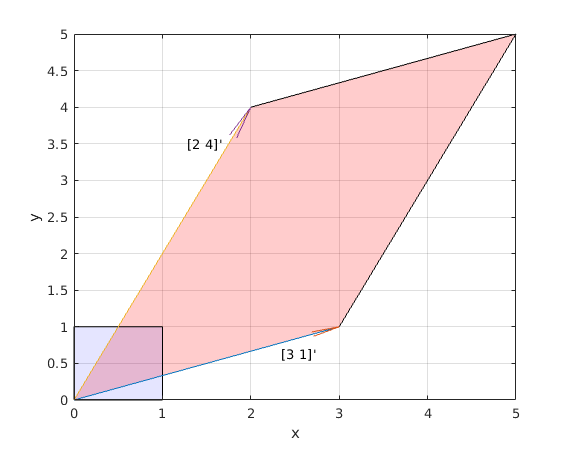
\includegraphics[scale=0.85]{resources/img/GeometryOfMatrices_images/linear_transformation.png}
	\end{center}
}


\date{\vspace{-6ex}}


\begin{document}
\searchableSubsection{\chapterTitle{Linear Algebra}}{linear algebra}{\bigskip\bigskip}

\searchableSubsection{\sectionTitle{Matrix Algebra}}{linear algebra}{\bigskip}

	\searchableSubsection{Basic properties of Matrix Algebra}{linear algebra}{\bigskip\bigskip
	
		\begin{definition}
		Matrix \textbf{equality} is defined component-wise so that if $A = B$ then $A$ and $B$ must have the same dimension as well as equal values in each component.
		\end{definition}
		\begin{definition}
		An \textbf{identity} element $e$ is defined as $ea = ae = a$.
		\end{definition}
		The definition of an identity element above is in any context (not just for matrices). For matrices this has certain consequences.
		\labeledProposition{Identity matrices must be square}{square_identity}
		\begin{proof}
		For a matrix $A$ and an identity matrix $I$, $AI = IA = A$ which means that $AI$, $IA$ and $A$ must all have the same dimensions. If $A$ is of dimension $m \times n$ then $I$ must have dimension $n \times m$ but then $AI$ has dimension $m \times m$ while $IA$ has dimension $n \times n$. We conclude that $m = n$ and both matrices are square.
		\end{proof}
		 
	
		\subsubsection{\small{If $A,B,C$ are matrices s.t. $AB = AC$, can we, in general, conclude that $B = C$?}}
		The answer is no, as the following example shows:
		\begin{align*}
			A = 
			\begin{pmatrix}
			0 & 0\\
			1 & 1\\
			\end{pmatrix},&&
			B = 
			\begin{pmatrix}
			1 & -1\\
			3 & 5\\
			\end{pmatrix},&&
			C = 
			\begin{pmatrix}
			8 & 0\\
			-4 & 4\\
			\end{pmatrix}
		\end{align*}
		\begin{align*}
		A = B = 
		\begin{pmatrix}
		0 & 0\\
		4 & 4\\
		\end{pmatrix}
		\end{align*}
		
		This is because multiplication by $A$ has no inverse (i.e. it's not a bijection and $A^{-1}$ does not exist) as we can see by the fact that $\vert{A}\vert = 0$.
		
		\subsubsection{\small{If $A,B,C$ are matrices s.t. $A + 5B = A + 5C$, can we, in general, conclude that $B = C$?}}
		The answer is yes because the matrix addition and scalar multiplication always have inverses. The inverse of $+ A$ is $- A$ and the inverse of scalar multiplication by $5$ is scalar multiplication by $\frac{1}{5}$. So we can say,
		\begin{align*}
		&& A + 5B &= A + 5C\\[8pt]
		&\iff & A + 5B - A &= A + 5C - A\\[8pt]
		&\iff & 5B &= 5C\\[8pt]
		&\iff & \left(\frac{1}{5}\right)5B &= \left(\frac{1}{5}\right)5C\\[8pt]
		&\iff & B &= C
		\end{align*}
		
		
		
		\subsubsection*{Matrix multiplication}
		Multiplication of matrices proceeds as a collection of dot-products of individual vectors. As a result, its properties are largely dependent on the properties of the dot-product. These are:
		\newcommand\vx{\V{x}}
		\newcommand\vy{\V{y}}
		\newcommand\vz{\V{z}}
		\begin{itemize}
		\item[]{If $\V{x} = (a, b)^{T}$ and $\V{y} = (e, g)^{T}$ then the dot-product $\langle \V{x}, \V{y} \rangle = ae + bg$ and,}
		\item{$\langle \vx, \vy \rangle = \langle \vy, \vx \rangle$}
		\item{$\alpha\langle \vx, \vy \rangle = \langle \alpha \vx, \vy \rangle = \langle \vx, \alpha \vy \rangle$}
		\item{$\langle \vx+\vy, \vz \rangle = \langle \vx, \vz \rangle + \langle \vy, \vz \rangle$}
		\item{$\langle \vx, \vx \rangle \geq 0$ and $\langle \vx, \vx \rangle = 0 \iff \vx = 0$}
		\end{itemize}
		
		Matrix multiplication treats the two operand matrices as collections of vectors with the first matrix having the vectors as rows and the second having the vectors as columns.
		\begin{align*}
			\begin{bmatrix}
			a & b \\
			c & d \\
			\end{bmatrix}
			\begin{bmatrix}
			e & f \\
			g & h \\
			\end{bmatrix}
			&=
			\begin{bmatrix}
			ae + bg & af + bh \\
			ce + dg & cf + dh \\
			\end{bmatrix}
		\end{align*}
		This difference in orientation of the vectors in the two operands results in the multiplication not being commutative - the order matters. So, the first property of the dot-product is not preserved but the others are preserved (albeit with a slight modification for the last one).
		\begin{align*}						
			\alpha
			\begin{bmatrix}
			a & b \\
			c & d \\
			\end{bmatrix}
			\begin{bmatrix}
			e & f \\
			g & h \\
			\end{bmatrix}
			&=
			\begin{bmatrix}
			\alpha a & \alpha b \\
			\alpha c & \alpha d \\
			\end{bmatrix}
			\begin{bmatrix}
			e & f \\
			g & h \\
			\end{bmatrix}
			=
			\begin{bmatrix}
			\alpha(ae + bg) & \alpha(af + bh) \\
			\alpha(ce + dg) & \alpha(cf + dh) \\
			\end{bmatrix}
			=
			\alpha
			\begin{bmatrix}
			ae + bg & af + bh \\
			ce + dg & cf + dh \\
			\end{bmatrix}		
		\end{align*}
		
		\begin{align*}
			\left(
			\begin{bmatrix}
			a & b \\
			c & d \\
			\end{bmatrix}
			+
			\begin{bmatrix}
			e & f \\
			g & h \\
			\end{bmatrix}
			\right)
			\begin{bmatrix}
			a+e & b+f\\
			c+g & d+h
			\end{bmatrix}
			&=
			\begin{bmatrix}
			i\,{\left(a+e\right)}+k\,{\left(b+f\right)} & j\,{\left(a+e\right)}+l\,{\left(b+f\right)}\\
			i\,{\left(c+g\right)}+k\,{\left(d+h\right)} & j\,{\left(c+g\right)}+l\,{\left(d+h\right)}\\
			\end{bmatrix}
		\end{align*}
		
		\begin{align*}
			\begin{bmatrix}
			a & b \\
			c & d \\
			\end{bmatrix}
			\begin{bmatrix}
			a & b \\
			c & d \\
			\end{bmatrix}^{T}
			=
			\begin{bmatrix}
			a & b \\
			c & d \\
			\end{bmatrix}
			\begin{bmatrix}
			a & c \\
			b & d \\
			\end{bmatrix}
			=
			\begin{bmatrix}
			a^{2} + b^{2} & ac + bd \\
			ac + bd & c^{2} + d^{2} \\
			\end{bmatrix}		
		\end{align*}
		\\\\
		So, to summarize:
		\begin{itemize}
		\item[]{If $A,B,C$ are matrices and $\alpha$ is a scalar then,}
		\item{$\alpha AB = (\alpha A)B = A(\alpha B) = \alpha(AB)$}
		\item{$(A + B)C = C(A + B) = AC + BC$}
		\item{$AA^{T}$ is a symmetric matrix with positive values along the diagonal}
		\end{itemize}
		
		\bigskip
		\subsubsection*{Matrix transpose}
		Denote the $i$th row of the matrix $A$ as $A[i:]$ and the $j$th column of the matrix $B$ as $B[j:]$ and a matrix whose components at $(i,j)$ are the dot-products of the $i$th row of the matrix $A$ with the $j$th column of the matrix $B$ as $(\langle A[i:], B[:j] \rangle)$. Then,
		\begin{align*}
		(AB)^{T} = (\langle A[i:], B[:j] \rangle)^{T} = (\langle A[j:], B[:i] \rangle) \\
		B^{T}A^{T} = (\langle B^{T}[i:], A^{T}[:j] \rangle) = (\langle B[:i], A[j:] \rangle)
		\end{align*}
		So, $(AB)^{T} = B^{T}A^{T}$. A consequence of this is that,
		\begin{align*}
		&& I = A\inv{A} &= (AA^{-1})^{T} = (A^{-1})^{T}A^{T} \\
		& \iff & I\inv{(A^{T})} &= (A^{-1})^{T}A^{T}\inv{(A^{T})} \\
		& \iff & \inv{(A^{T})} &= (A^{-1})^{T}
		\end{align*}
		
		\bigskip
		\subsubsection*{Matrix inverse}
		\begin{definition}
		Inverse property is if $ \exists \text{ a matrix } B \suchthat AB = BA = I $ then $B$ is the \textbf{inverse} of $A$.
		\end{definition}
		This definition is inherently bound up with the definition of the identity ($\exists \text{ a matrix } I \suchthat AI = IA = A$) and both define the identity and inverse elements as commutatively producing their result under matrix multiplication. Since matrix multiplication is not, in general, commutative there is no guarantee that if $AB = I$ then $BA = I$. An example of this failing is,
		\begin{align*}
			A = 
			\begin{bmatrix}
			1 & 2 \\
			\end{bmatrix},\;
			&B =
			\begin{bmatrix}
			1 \\
			0 \\
			\end{bmatrix}
			\\[10pt]
			AB = 
			\begin{bmatrix}
			1 \\
			\end{bmatrix} = I_1,\;
			&BA =
			\begin{bmatrix}
			1 & 2 \\
			0 & 0 \\
			\end{bmatrix} \neq I_2
		\end{align*}
		
		But we could have guessed this because \autoref{prop:square_identity} showed that identity matrices must be square and its product with a matrix must be defined from both the left and the right, i.e. $IA = AI = A$ meaning that the matrix $A$ must have the same dimensions as $I$. So, for non-square matrices, no identity can exist. If there is no identity, then the inverse is not defined either.
		
		\labeledProposition{If the inverses of the matrices $A$ and $B$ both exist then so does the inverse of the product $AB$ and it is equal to $\inv{B}\inv{A}$.}{existence_inverse_product}
		\begin{proof}
		\begin{align*}
		& 	  &	(AB)\inv{(AB)} &= I \\
		&\iff &	(\inv{A}A)B\inv{(AB)} &= \inv{A}I \\
		&\iff &	(\inv{B}B)\inv{(AB)} &= \inv{B}\inv{A} \\
		&\iff &	\inv{(AB)} &= \inv{B}\inv{A} \\
		\end{align*}
		and since $\inv{B}$ and $\inv{A}$ both exist then their product exists.
		Furthermore, this holds for a product of any finite sequence of invertible matrices $A_1A_2\cdots A_n$ which can easily be shown by induction on the associative product.
		\end{proof}
	}
	
	\searchableSubsection{Matrices as linear transformations}{linear algebra}{\bigskip
		
		\subsubsection{Multiplying a vector by a matrix on the left: $ A\V{x} = \V{y} $}
		Left multiplication of a matrix $A$ of dimension $m \times n$ on a column vector $\V{x}$ of dimension $n \times 1$ transforms it to a column vector $\V{y}$ of dimension $m \times 1$.
		\begin{align*}
			\begin{bmatrix}
			a_{11} & \cdots & a_{1n} \\
			\vdots & \vdots & \vdots \\
			a_{m1} & \cdots & a_{mn} \\
			\end{bmatrix}
			\begin{bmatrix}
			x_1 \\
			\vdots \\
			\vdots \\
			x_n \\
			\end{bmatrix}
			=
			\begin{bmatrix}
			y_1 \\
			\vdots \\
			y_m \\
			\end{bmatrix}
		\end{align*}
		This can be thought of a function from the space of n-dimensional vectors from which $\V{x}$ is drawn to the space of m-dimensional vectors in which $\V{y}$ resides. So, for real-valued vectors, the function would be a function \mbox{$f:\R{n} \mapsto \R{m}$} such that,
		\[ f(x_1,\cdots,x_n) = \V{y} =
					\begin{bmatrix}
					y_1 \\
					\vdots \\
					y_m \\
					\end{bmatrix} \]
		Or else, this could be thought of as $m$ n-ary functions of the form $f:\R{n} \mapsto \R{}$,
		\begin{align*}
		f_1(x_1,\cdots,x_n) &= a_{11}x_1 + \cdots + a_{1n}x_n = y_1 \\
		\vdots \\
		f_m(x_1,\cdots,x_n) &= a_{m1}x_1 + \cdots + a_{mn}x_n = y_m \\
		\end{align*}
		In this case, each row of the matrix is a real-valued function in $n$ variables. Each of these functions is \textit{homogenous linear} (a function of the form $a_1x_1 + \cdots + a_kx_k + c$ for scalars $a_1,\cdots,a_k,c$ and $c = 0$) and so the system of functions is called a \textit{linear transformation}.\\
		
		\subsubsection{Multiplying a matrix of vectors by a matrix on the left: $ AX = Y $}
		Looking at the matrix as a linear transformation from one co-ordinate space to another, consider $AX = Y$ where $X$ is a matrix - which may be considered a collection of vectors - transformed by the matrix $A$ into the matrix - or collection of vectors - $Y$.\\
					
		\exampleMatrixTwoDTransform
		
		\subsubsection{Types of Transformations}
		There are 3 basic types of transformation:
		\begin{itemize}
		\item{\textbf{Rigid body} - preserves distances and angles.
			\subitem{Examples: translation and rotation.}
		}
		\item{\textbf{Conformal} - preserves angles.
			\subitem{Examples: translation, rotation and uniform scaling.}
		}
		\item{\textbf{Affine} - preserves parallelism.
			\subitem{Examples: translation, rotation, uniform and non-uniform scaling, shearing and reflection.}
		}
		\end{itemize}
		
		\subsubsection{Rigid Body}
		\subparagraph{Translation}
		So as to perform the translation as multiplication by a transformation matrix we take the approach of homogeneous coordinates (see:\url{https://en.wikipedia.org/wiki/Homogeneous_coordinates}) so we form matrix with the identity in the first two columns and then a third column with the translation vector. Then, we add a row of ones to the vectors we will translate.
		
		\begin{align*}
		A =
		\begin{bmatrix}    
		1 & 0  & 3 \\
		0 & 1  & 4 \\		
		\end{bmatrix}
		,\; X = 
		\begin{bmatrix}  
		0   &  1  &   1  &   0 \\
		0   &  0  &   1  &   1	\\	
		1   &  1  &   1  &   1	\\	
		\end{bmatrix} \\[10pt]
		AX = Y = 
		\begin{bmatrix}   
		3  &   4  &   4  &   3 \\
		4  &   4  &   5  &   5	\\
		\end{bmatrix}
		\end{align*}
		
		\begin{center}
		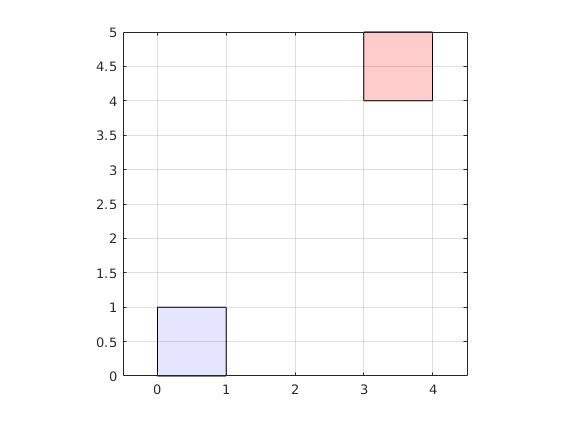
\includegraphics[scale=0.85]{resources/img/GeometryOfMatrices_images/translation.png}
		\end{center}
		
		\subparagraph{Rotation}
		\begin{align*}
		A =
		\begin{bmatrix}    
		\cos{\theta}  &  -\sin{\theta} \\
		\sin{\theta}  &  \cos{\theta} \\		
		\end{bmatrix}
		,\; X = 
		\begin{bmatrix}  
		0   &  1  &   1  &   0 \\
		0   &  0  &   1  &   1	\\	
		\end{bmatrix} \\[10pt]
		AX = Y = 
		\begin{bmatrix}   
		0  &   0.5253  &  -0.3256  &  -0.8509 \\
		0  &   0.8509  &   1.3762  &   0.5253	\\
		\end{bmatrix}
		\end{align*}
	
		\begin{center}
		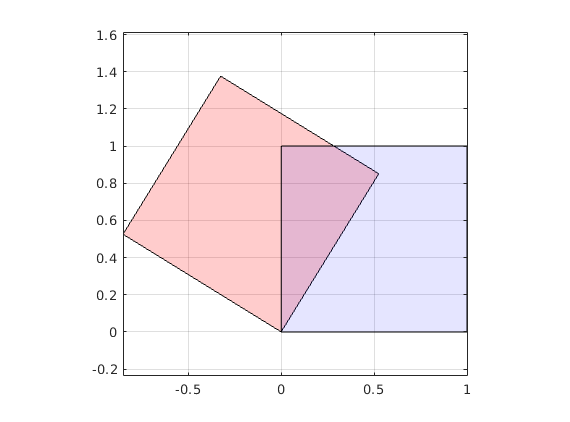
\includegraphics[scale=0.85]{resources/img/GeometryOfMatrices_images/rotation.png}
		\end{center}
		
		\subsubsection{Conformal}
		\subparagraph{Uniform Scaling}
		\begin{align*}
		A =
		\begin{bmatrix}    
		3  &  0 \\
		0  &  3 \\		
		\end{bmatrix}
		,\; X = 
		\begin{bmatrix}  
		0   &  1  &   1  &   0 \\
		0   &  0  &   1  &   1	\\	
		\end{bmatrix} \\[10pt]
		AX = Y = 
		\begin{bmatrix}   
		0  &   3  &  3  &  0 \\
		0  &   0  &  3  &  3 \\
		\end{bmatrix}
		\end{align*}
	
		\begin{center}
		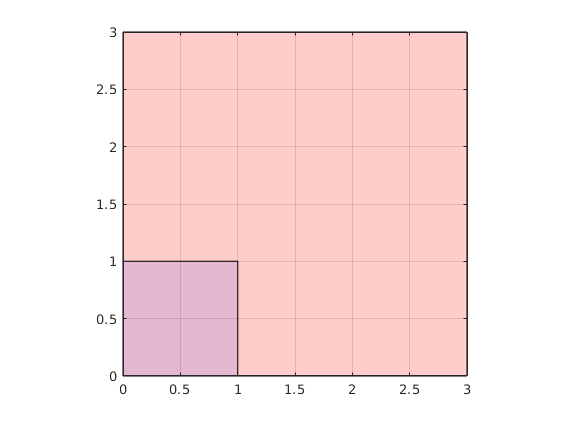
\includegraphics[scale=0.85]{resources/img/GeometryOfMatrices_images/uniform_scaling.png}
		\end{center}
		
		\subsubsection{Affine}
		\subparagraph{Non-uniform Scaling}
		\begin{align*}
		A =
		\begin{bmatrix}    
		2  &  0 \\
		0  &  3 \\		
		\end{bmatrix}
		,\; X = 
		\begin{bmatrix}  
		0   &  1  &   1  &   0 \\
		0   &  0  &   1  &   1	\\	
		\end{bmatrix} \\[10pt]
		AX = Y = 
		\begin{bmatrix}   
		0  &   2  &  2  &  0 \\
		0  &   0  &  3  &  3 \\
		\end{bmatrix}
		\end{align*}
	
		\begin{center}
		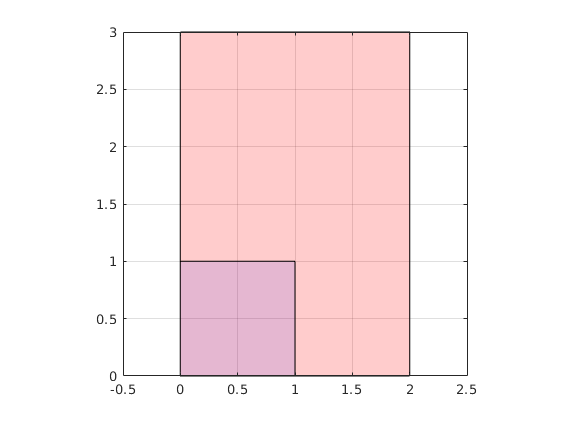
\includegraphics[scale=0.85]{resources/img/GeometryOfMatrices_images/non_uniform_scaling.png}
		\end{center}
		
		\subparagraph{Shearing}
		\begin{align*}
		A =
		\begin{bmatrix}    
		1  &  1 \\
		0  &  1 \\		
		\end{bmatrix}
		,\; X = 
		\begin{bmatrix}  
		0   &  1  &   1  &   0 \\
		0   &  0  &   1  &   1	\\	
		\end{bmatrix} \\[10pt]
		AX = Y = 
		\begin{bmatrix}   
		0  &   1  &  2  &  1 \\
		0  &   0  &  1  &  1 \\
		\end{bmatrix}
		\end{align*}
	
		\begin{center}
		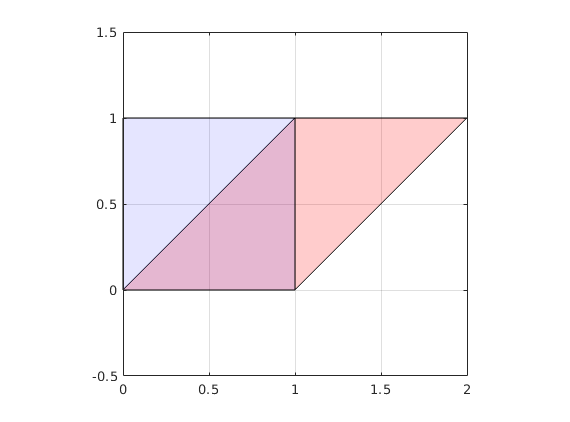
\includegraphics[scale=0.85]{resources/img/GeometryOfMatrices_images/shearing1.png}
		\end{center}
		
		\begin{align*}
		A =
		\begin{bmatrix}    
		1  &  1 \\
		0.2  &  1 \\		
		\end{bmatrix}
		,\; X = 
		\begin{bmatrix}  
		0   &  1  &   1  &   0 \\
		0   &  0  &   1  &   1	\\	
		\end{bmatrix} \\[10pt]
		AX = Y = 
		\begin{bmatrix}   
		0  &   1  &  2  &  1 \\
		0  &   0.2  &  1.2  &  1 \\
		\end{bmatrix}
		\end{align*}
	
		\begin{center}
		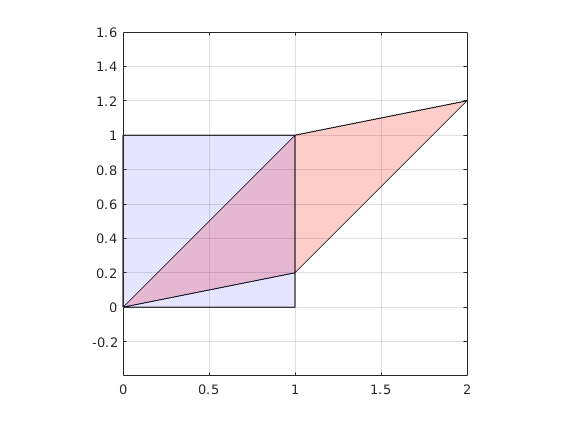
\includegraphics[scale=0.85]{resources/img/GeometryOfMatrices_images/shearing2.png}
		\end{center}
		
		\subparagraph{Reflection}
		\begin{align*}
		A =
		\begin{bmatrix}    
		1  &  0 \\
		0  &  -1 \\		
		\end{bmatrix}
		,\; X = 
		\begin{bmatrix}  
		0   &  1  &   1  &   0 \\
		0   &  0  &   1  &   1	\\	
		\end{bmatrix} \\[10pt]
		AX = Y = 
		\begin{bmatrix}   
		0  &   1  &  1  &  0 \\
		0  &   0  &  -1  &  -1 \\
		\end{bmatrix}
		\end{align*}
	
		\begin{center}
		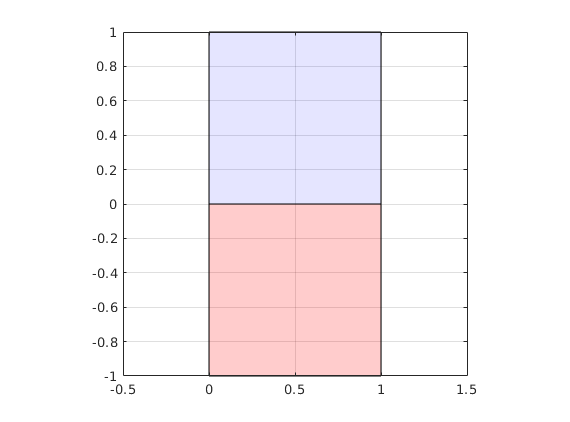
\includegraphics[scale=0.85]{resources/img/GeometryOfMatrices_images/reflection.png}
		\end{center}
	}
	
	\pagebreak
	\searchableSubsection{Elementary Matrices and Row Operations}{linear algebra}{\bigskip
		\notation{The \textbf{matrix units} - matrices with a single non-zero component whose value is 1 are traditionally named $\bm{e_{ij}}$ where $i,j$ is the matrix co-ordinate of the 1.}\\\\
		An arbitrary matrix $A = (a_{ij})$ may be expressed as a sum of such unit matrices as $A = a_{11}e_{11} + \cdots + a_{nn}e_{nn}$.
		\[
		e_{ij} = 
		\begin{bmatrix}
		\cdots & \cdots & \cdots \\
		\vdots & \vdots & \vdots \\
		\cdots & 1 & \cdots \\
		\vdots & \vdots & \vdots \\
		\cdots & \cdots & \cdots \\
		\end{bmatrix}
		\]
		So matrix units can be used to analyse matrix addition but to analyse matrix multiplication some square matrices called \textbf{elementary matrices} are more useful.\\
		
		Multiplying a matrix from the left (so doing row operations), there are 3 types of elementary matrix:
		\subsubsection*{Adding rows: $\bm{ I + ae_{ij}\;\;\;\; \text{ for } i \neq j }$}
			\[
			\begin{bmatrix}
			1 	&  &  	&	\\
			 	& \cdot & a & \\
			 	&  & \cdot & 	\\
			 	&  & 	& 1	\\
			\end{bmatrix}
			\]
			This adds $a$ times some row to another row.
			
		\subsubsection*{Swapping rows: $\bm{ I + e_{ij} + e_{ji} - e_{ii} - e_{jj}\;\;\;\; \text{ for } i \neq j }$}
			\[
			\begin{bmatrix}
			1 	&  &  	&	\\
			 	& 0 & 1 & \\
			 	& 1 & 0 & 	\\
			 	&  & 	& 1	\\
			\end{bmatrix}
			\]
			This swaps the rows $i$ and $j$.
		
		\subsubsection*{Scalar-multiplying a row: $\bm{ I + (c - 1)e_{ii}\;\;\;\; \text{ for } c \neq 0 }$}
			\[
			\begin{bmatrix}
			1 	&  &  	&	\\
			 	& \cdot &  & \\
			 	&  & c 	& 	\\
			 	&  & 	& 1	\\
			\end{bmatrix}
			\]
			This multiplies row $i$ by $c$.
		
		\bigskip	
		\labeledProposition{Elementary matrices are invertible and their inverses are also elementary matrices.}{elementary_invertible}
		\begin{proof} Proceed by cases on the 3 elementary types of elementary matrices.
		~\paragraph{Case $\bm{ I + ae_{ij} }$}  If $R_i$ is row $i$ and $R_j$ is row $j$, then this matrix performs $R_i + aR_j$. Clearly this can be "undone" by performing $R_i - aR_j$. So the matrix, $I - ae_{ij}$ is the inverse and clearly this is also an elementary matrix of the same type.
		\paragraph{Case $\bm{ I - e_{ii} - e{jj} + e_{ij} + e_{ji} }$} This matrix swaps 2 rows in a permutation that is its own inverse.
		\paragraph{Case $\bm{ I + (c - 1)e_{ii} }$} This matrix performs $cR_i$ and so it is "undone" by performing $\inv{c}R_i$ (which for a real-valued matrix would be $\left(\frac{1}{c}\right)R_i$) and this inverse matrix is also an elementary matrix of the same type. 
		\end{proof}
		
		\bigskip
		\labeledProposition{Suppose $AX = B$ and a series of elementary row operations on $[A \;\vert\; B]$ produces $[A' \;\vert\; B']$, then the solutions of $A'X = B'$ are the same as those of $AX = B$.}{row_reduced_equivalence}
		\begin{proof}
		First note that the series of elementary row operations is described as multiplication on the left by a series of elementary matrices say, $E_1, E_2, \cdots , E_n$ so that,
		\[ [A' \;\vert\; B'] = [(E_n\cdots E_2E_1)A \;\vert\; (E_n\cdots E_2E_1)B] \]
		Now, let $(E_n\cdots E_2E_1) = E$ and notice that, since each of the individual $E_i$ is invertible the product of them is also invertible by \autoref{prop:existence_inverse_product} so,
		\[ A'X = B' \iff EAX = EB \]
		and the existence of the inverse $E^{-1}$ means that the law of cancellation is in effect so,
		\[ EAX = EB \iff AX = B \]
		\[ \therefore A'X = B' \iff AX = B \]
		\end{proof}
		
		\labeledProposition{Let $A$ be a square matrix. The following conditions are equivalent:
			\begin{itemize}
			\item{$A$ can be reduced to the identity by a sequence of elementary row operations.}
			\item{$A$ is a product of elementary matrices.}
			\item{$A$ is invertible.}
			\item{The system of homogeneous equations $AX = 0$ has only the trivial solution $X = 0$.}
			\end{itemize}		
		}{matrix_equivalent_properties}
		\begin{proof}
			If $A$ can be reduced to the identity by a sequence of elementary row operations then,
			\[ (E_n\cdots E_2E_1)A = I \]
			and by \autoref{prop:elementary_invertible} and \autoref{prop:existence_inverse_product} the matrix $(E_n\cdots E_2E_1)$ is invertible so,
			\[ A = \inv{(E_n\cdots E_2E_1)}I = \inv{(E_n\cdots E_2E_1)} = \inv{E_1}\inv{E_2}\cdots \inv{E_n} \]
			and, also by \autoref{prop:elementary_invertible}, $A$ is a product of elementary matrices and is invertible.\\
			Furthermore, if $AX = 0$ then $X = \inv{A}0 = 0$ - i.e. the only solution to $AX = 0$ is $X = 0$.
		\end{proof}
	}
	
	
	
	\pagebreak
	\searchableSubsection{Determinants}{linear algebra}{\bigskip
		The determinant of a $1 \times 1$ matrix is just its unique component entry,
		\[ det
		\begin{bmatrix}
		{a}\\
		\end{bmatrix} 
		= a \]
		and the determinant of a $2 \times 2$ matrix is given by the formula,
		\[ det 
		\begin{bmatrix}
		a & b \\
		c & d \\
		\end{bmatrix}
		= ad - bc \]
		\\
		Returning to our example of a 2d operator:\\
		
		\exampleMatrixTwoDTransform
		
		We see that $det\; A = 10$ and the parallelogram, $Y$, that is the image of the unit square, $X$, under the transformation represented by $A$ has area,
		\[ \text{area } = b \cdot h = \vert\langle 3, 1 \rangle \vert \cdot \vert \langle 2-3, 4-1 \rangle\vert = \sqrt{10} \cdot \sqrt{10} = 10 \]
	}
	
	
	\pagebreak
	\searchableSubsection{Relations on matrices}{linear algebra}{\bigskip\bigskip
	
		\searchable{subsubsection}{\small{Let $X$ be the set of $n \times n$ real matrices. Define a relation $\sim$ on $X$ by:
			\[ M \sim N \iff \exists \text{ an invertible } P \in X \suchthat N = P^{-1}MP. \]
		Prove that $\sim$ is an equivalence relation.
		}}{linear algebra, equivalence relations}{
		\paragraph{Reflexivity:}
		\begin{align*}
		& N = I^{-1}NI \\
		\therefore \; & N \sim N
		\end{align*}
		
		\paragraph{Symmetry:}
		\begin{align*}
		& & N &= P^{-1}MP \\
		&\iff & NP^{-1} &= P^{-1}M(PP^{-1}) \\
		&\iff & NP^{-1} &= P^{-1}M \\
		&\iff & PNP^{-1} &= (PP^{-1})M \\
		&\iff & PNP^{-1} &= M \\
		&\iff & R^{-1}NR &= M,\;\; R \in X\\
		&\;\;\therefore & N \sim M &\iff M \sim N
		\end{align*}
		
		\paragraph{Transitivity:}
		\begin{align*}
		& & N &= P^{-1}MP,\;\; M = Q^{-1}AQ \\
		&\implies & N &= P^{-1}(Q^{-1}AQ)P \\
		&\iff & N &= (P^{-1}Q^{-1})A(QP) \\
		&\iff & N &= R^{-1}AR,\;\; R \in X\\
		&\;\;\therefore & (N \sim M) & \wedge (M \sim Q) \iff (N \sim Q)
		\end{align*}
		}
	}
	
\end{document}